\documentclass{article}
\usepackage[utf8]{inputenc}
\usepackage{graphicx}
\usepackage{amsmath}
\usepackage{amsfonts}
\usepackage{amsbsy}
\usepackage{mathrsfs}
\usepackage{appendix}
\usepackage{amsthm}
\usepackage{bbold}
\usepackage{epstopdf}

\newcommand{\bs}[1]{\boldsymbol{#1}}
\newcommand{\bb}[1]{\mathbf{#1}}
\newcommand{\pd}[2]{\frac{\partial {#1}}{\partial {#2}}}
\newcommand{\parti}[1]{\pd{}{#1}}

\title{TP1 for Proba Graph}
\author{Leman FENG\\ Email: flm8620@gmail.com\\Website: lemanfeng.com}

\begin{document}
	\maketitle
	\section{Problem 1}
	
	Let's say we have observations $(z_1,x_1) \dots (z_n,x_n)$. By definition, the likelihood of this sample w.r.t parameter $\bs{\pi},\bs{\theta}$ is:
	$$
	\prod_{i=1}^n \mathbb{P}_{(\bs{\pi},\bs{\theta})}(z=z_i,x=x_i) = 
	\prod_{i=1}^n \mathbb{P}_{(\bs{\pi},\bs{\theta})}(x=x_i | z=z_i) \mathbb{P}_{(\bs{\pi},\bs{\theta})}(z=z_i)=
	\prod_{i=1}^n \pi_{z_i} \theta_{z_ix_i}
	$$
	
	Maximize likelihood:
	\begin{equation*}
	\begin{split}
	(\hat{\bs{\pi}},\hat{\bs{\theta}}) &= \arg\max \sum_{i=1}^n \log \mathbb{P}_{(\bs{\pi},\bs{\theta})}(z=z_i,x=x_i)\\
	&= \arg\max \sum_{i=1}^n \log \pi_{z_i} \theta_{z_ix_i}
	\end{split}
	\end{equation*}
	
	Use method of Lagrange multipliers, set multiplier $\lambda$ and $\mu_j, j=1\dots M$
	$$
	L = \sum_{i=1}^n \log \pi_{z_i} \theta_{z_ix_i} - \lambda (\sum_{j=1}^M \pi_j - 1) - \sum_{j=1}^M \mu_j (\sum_{l=1}^K \theta_{jl} - 1)
	$$
	
	Then
	$$
	\pd{L}{\theta_{mk}} = \sum_{i=1}^n \frac{\mathbb{1}\{z_i=m,x_i=k\}}{\theta_{z_ix_i}} - \mu_m = 0, \  \forall m,k
	$$
	$$
	\pd{L}{\pi_m} = \sum_{i=1}^n \frac{\mathbb{1}\{z_i=m\}}{\pi_{z_i}} - \lambda = 0, \  \forall m
	$$
	
	Or rewritten as:
	$$
	\pd{L}{\theta_{mk}} = \frac{\#\{i,z_i=m,x_i=k\}}{\theta_{mk}} - \mu_m = 0, \  \forall m,k
	$$
	$$
	\pd{L}{\pi_m} = \frac{\#\{i,z_i=m\}}{\pi_m} - \lambda = 0, \  \forall m
	$$
	
	Then we can see the proportionalities:
	$$
	\frac{\#\{i,z_i=m,x_i=k\}}{\mu_m} = \theta_{mk}, \  \forall m,k
	$$
	$$
	\frac{\#\{i,z_i=m\}}{\lambda} = \pi_m, \  \forall m
	$$
	
	Notice that
	$$
	\sum_{m=1}^K \theta_{ml} = 1, \ \sum_{m=1}^M \pi_m = 1
	$$
	
	So
	$$
	\hat{\pi_i} = \frac{\#\{i,z_i=m\}}{n}, \ \hat{\theta_{mk}} = \frac{\#\{i,z_i=m,x_i=k\}}{\#\{i,z_i=m\}}
	$$
	
	\section{Problem 2.1}
	\subsection{Question (a)}
	Let's say we observed $(x_1,y_1), \dots, (x_n,y_n)$, log-likelihood is
	\begin{equation*}
	\begin{split}
	l((x_i,y_i)_i) &= \sum_{i=1}^n \log p_{(\pi,\mu_0,\mu_1,\Sigma)}(x_i,y_i)\\
	&=\sum_{i,y_i=1} [\log \pi -\log((2\pi)^\frac{N}{2} |\Sigma|^\frac{1}{2}) - \frac{1}{2} (x_i-\mu_0)^T \Sigma^{-1} (x_i-\mu_0) ]\\
	&+\sum_{i,y_i=0} [\log (1-\pi) -\log((2\pi)^\frac{N}{2} |\Sigma|^\frac{1}{2}) - \frac{1}{2} (x_i-\mu_0)^T \Sigma^{-1} (x_i-\mu_0) ]\\
	&= - \frac{N}{2} n \log(2\pi) + \frac{n}{2} \log|\Sigma^{-1}| + \sum_{i,y_i=1} \log \pi -\frac{1}{2} \sum_{i,y_i=1}(x_i^T\Sigma^{-1}x_i-2x_i^T\Sigma^{-1}\mu_0+\mu_0^T\Sigma^{-1}\mu_0)\\
	&+ \sum_{i,y_i=0} \log (1-\pi) -\frac{1}{2} \sum_{i,y_i=0}(x_i^T\Sigma^{-1}x_i-2x_i^T\Sigma^{-1}\mu_1+\mu_1^T\Sigma^{-1}\mu_1)
	\end{split}
	\end{equation*}
	
	Note $n_0 = \#\{i,y_i=0\}$ and $n_1 = \#\{i,y_i=1\}$, we can see function $l$ is concave because it's sum of several concave functions, so its maximum can be found by taking derivative, we know that $\pd{\log|A|}{A} = A^{-1}$:
	\begin{equation*}
	\begin{split}
	\pd{l}{\pi} &= \frac{n_0}{1-\pi} - \frac{n_1}{\pi} = 0\\
	\pd{l}{\mu_0} &= \sum_{i,y_i=0} (\Sigma^{-1} x_i - \Sigma^{-1} \mu_0) = 0\\
	\pd{l}{\mu_1} &= \sum_{i,y_i=1} (\Sigma^{-1} x_i - \Sigma^{-1} \mu_1) = 0\\
	\pd{l}{\Sigma^{-1}} &=  -\frac{1}{2} \sum_{i,y_i=0} (x_i-\mu_0) (x_i-\mu_0)^T -\frac{1}{2} \sum_{i,y_i=1} (x_i-\mu_1) (x_i-\mu_1)^T + \frac{n}{2} \Sigma = 0
	\end{split}
	\end{equation*}
	
	We can get:
	\begin{equation} \label{LDAresult}
	\begin{split}
	\hat{\pi} &= \frac{n_1}{n}\\
	\hat{\mu}_0 &= \frac{1}{n_0} \sum_{i,y_i=0} x_i  = \text{sample mean of}\ \{x_i|y_i=0\}\\
	\hat{\mu}_1 &= \frac{1}{n_1} \sum_{i,y_i=1} x_i  = \text{sample mean of}\ \{x_i|y_i=1\}\\
	\end{split}
	\end{equation}
	Take $\hat{\mu}_0,\hat{\mu}_1$ into $\pd{l}{\Sigma^{-1}}$. So
	$$
	\hat{\Sigma} = \frac{1}{n} \sum_{i,y_i=0} (x_i-\hat{\mu}_0) (x_i-\hat{\mu}_0)^T + \frac{1}{n} \sum_{i,y_i=1} (x_i-\hat{\mu}_1) (x_i-\hat{\mu}_1)^T
	$$
	We note $Q_k$ as the sample biased estimate of covariance for $\{x_i|y_i=k\}$
	$$
	Q_k = \frac{1}{n_k}\sum_{i,y_i=k} (x_i-\hat{\mu}_k) (x_i-\hat{\mu}_k)^T
	$$
	Then $\hat{\Sigma}$ is actually weighted sum of $Q_1,Q_0$:
	$$
	\hat{\Sigma} = \frac{n_0}{n} Q_0 + \frac{n_1}{n} Q_1
	$$
	
	\subsection{Question (b)}
	By Bayes rule:
	\begin{equation*}
	\begin{split}
	p(y=1|x) &= \frac{p(x,y=1)}{p(x)}=\frac{p(x|y=1)p(y=1)}{p(x|y=1)p(y=1) + p(x|y=0)p(y=0)}\\
	&=\frac{1}{1+\frac{p(y=0)}{p(y=1)} \frac{p(x|y=0)}{p(x|y=1)}} = \frac{1}{1+\frac{1-\pi}{\pi}\exp(- \frac{1}{2} (x-\mu_0)^T \Sigma^{-1} (x-\mu_0) + \frac{1}{2} (x-\mu_1)^T \Sigma^{-1} (x-\mu_1))}\\
	&= \frac{1}{1+\frac{1-\pi}{\pi}\exp(-x\Sigma^{-1}(\mu_1-\mu_0) - \frac{1}{2} (\mu_0^T\Sigma^{-1}\mu_0-\mu_1^T\Sigma^{-1}\mu_1))}\\
	&= \frac{1}{1+\exp(-x\Sigma^{-1}(\mu_1-\mu_0) - \frac{1}{2} (\mu_0^T\Sigma^{-1}\mu_0-\mu_1^T\Sigma^{-1}\mu_1) - \log (\frac{\pi}{1-\pi}) )}\\
	&= \sigma(w^T x + b)
	\end{split}
	\end{equation*}
	where $\sigma(x) = \frac{1}{1+e^{-x}}$ is the sigmoide function. And
	\begin{equation}\label{LDA}
	w = (\mu_1-\mu_0)^T\Sigma^{-1}, b=\frac{1}{2} (\mu_0^T\Sigma^{-1}\mu_0-\mu_1^T\Sigma^{-1}\mu_1) + \log (\frac{\pi}{1-\pi})
	\end{equation}
	\subsection{Question (c)}
	Result:
	
	Class A : $w = [-6.622,-9.346],\ b=-0.136$
	
	Class B : $w = [-1.921,0.954],\ b=9.293e-04$
	
	Class C : $w = [-2.051,-0.273],\ b=0.112$
	
	See Figure \ref{fig:a},\ref{fig:b},\ref{fig:c}
	
	
	\section{Problem 2.2}
	\subsection{Question (a)}
	Result:
	
	Class A : $w = [-1.47e+03,-2.54e+03],\ b=-2.61e+02$
	
	Class B : $w = [-1.705,1.024],\ b=1.350$
	
	Class C : $w = [-2.203,0.709],\ b=0.959$
	\subsection{Question (b)}
	
	See Figure \ref{fig:a},\ref{fig:b},\ref{fig:c}
	

	\section{Problem 2.3}
	\subsection{Question (a)}
	Notice that in Linear Regression $b$ need to be subtracted by $0.5$ to be compare with other two methods.
	
	Result:
	
	Class A : $w = [-0.264;-0.373],\ b=0.492$
	
	Class B : $w = [-0.104;0.052],\ b=5.043e-05$
	
	Class C : $w = [-0.128;-0.017],\ b=0.0084$
	\subsection{Question (b)}
	Question is not well posed. We should ask to plot the line define by equation
	$$
	p(y>0.5|x) = 0.5
	$$
	
	
	See Figure \ref{fig:a},\ref{fig:b},\ref{fig:c}
	\begin{figure}
		\centering
		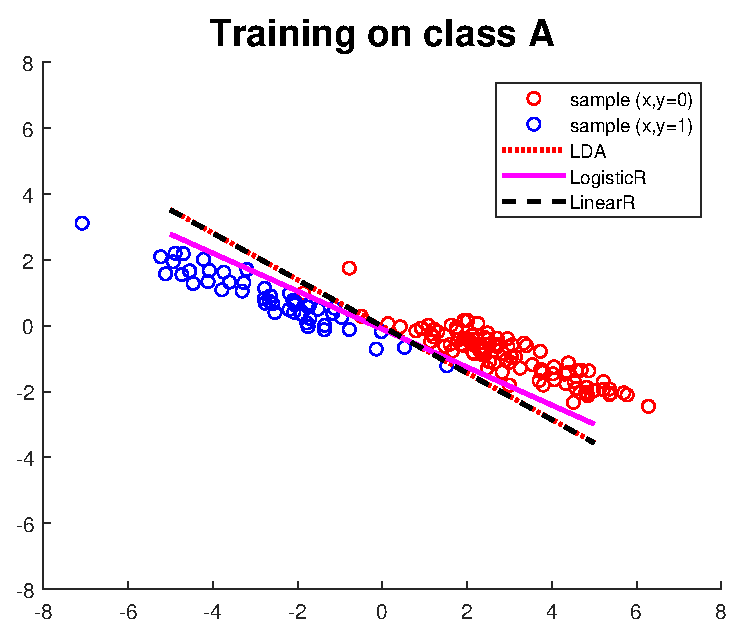
\includegraphics[scale=0.6]{plot_a.eps}
		\caption{Training on class A}
		\label{fig:a}
	\end{figure}
	\begin{figure}
		\centering
		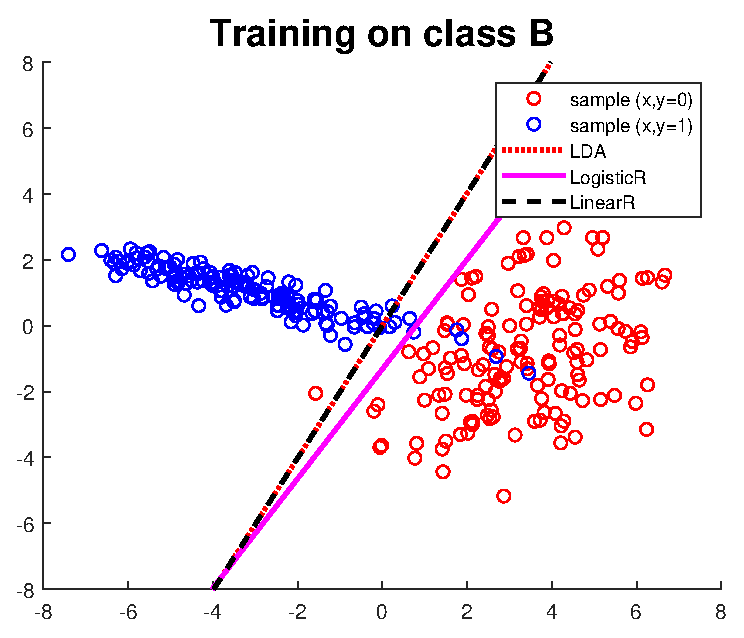
\includegraphics[scale=0.6]{plot_b.eps}
		\caption{Training on class B}
		\label{fig:b}
	\end{figure}
	\begin{figure}
		\centering
		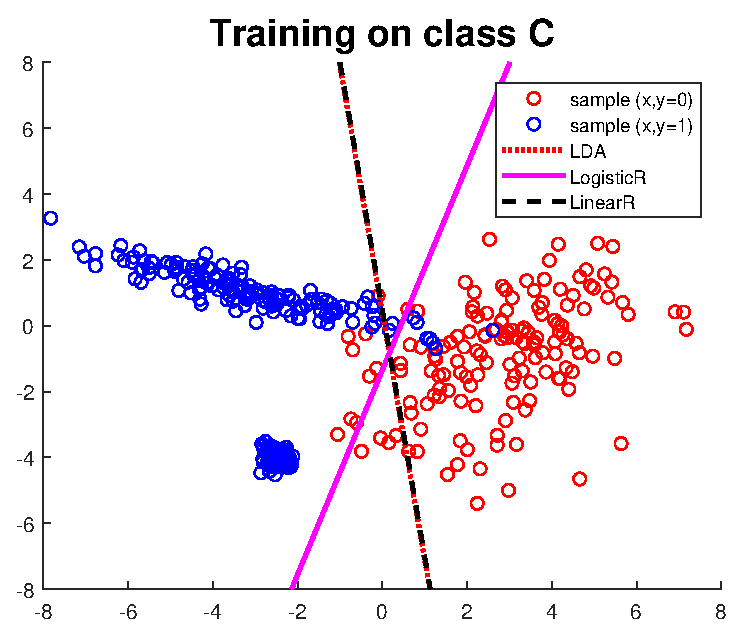
\includegraphics[scale=0.6]{plot_c.eps}
		\caption{Training on class C}
		\label{fig:c}
	\end{figure}

	\section{Problem 2.4}
	\subsection{Question (a)}
	Error:
	\begin{center}
		\begin{tabular}{ c | c | c | c | c | c | c }
			\hline
			 & A train & A test & B train & B test & C train & C test \\ \hline
			LDA & 2/1500 & 30/1500 & 9/300 & 83/2000 & 22/400 & 127/3000 \\ \hline
			Logistic & 0/1500 & 53/1500 & 6/300 & 86/2000 & 16/400 & 68/3000  \\ \hline
			Linear & 2/1500 & 31/1500 & 9/300 & 83/2000 & 22/400 & 127/3000  \\ \hline
		\end{tabular}
	\end{center}

	\subsection{Question (b)}
	Of course test error are normally larger than training error. So we should only compare test error.
	
	On dateset A, LDA and Linear has better performance than Logistic, because the dataset is nearly two gaussian distribution with same covariance. LDA model is more correct.
	
	On dataset B, they have basically same performance. Because dataset is nearly two gaussian distribution with different covariances.
	
	On dateset C, Logistic has better performance because there are nearly three gaussian in data. So assuming blue dots in Figure \ref{fig:c} is one gaussian makes no sense.
	
	We can see LDA and Linear Regression give same classifier. Except for a small difference in test A, which should be caused by numerical errors. We can show that in this case, LDA and Linear Regression are equivalent:
	
	W.l.o.g, we assume data is centered. For LDA, $n_0 \hat{\mu}_0=n_1 \hat{\mu}_1$ according to Equation \ref{LDAresult}. For Linear Regression, we have:
	$$
	\hat{w}_L = (X^T X)^{-1} X^T y
	$$
	
	$(X^T X)^{-1}$ is proportional to empirical covariance of all observation. For LDA, $\hat{\Sigma}$ is weighted empirical covariance of respectively two type of data. By assumption of centered data, with the parallel axis theorem of momentum, we can say these two terms are proportional.
	
	Then $X^T y$ is just sum of $\{x_i|y_i=1\}$, which is proportional to $\hat{\mu_1}$ again. So $w$ given by LDA and Linear Regression are proportional. So they are equivalent in this case.
	\section{Problem 2.5}
	\begin{equation*}
	\begin{split}
	l((x_i,y_i)_i) &= \sum_{i=1}^n \log p_{(\pi,\mu_0,\mu_1,\Sigma_0,\Sigma_1)}(x_i,y_i)\\
	&=\sum_{i,y_i=1} [\log \pi -\log((2\pi)^\frac{N}{2} |\Sigma_1|^\frac{1}{2}) - \frac{1}{2} (x_i-\mu_0)^T \Sigma_1^{-1} (x_i-\mu_0) ]\\
	&+\sum_{i,y_i=0} [\log (1-\pi) -\log((2\pi)^\frac{N}{2} |\Sigma_0|^\frac{1}{2}) - \frac{1}{2} (x_i-\mu_0)^T \Sigma_0^{-1} (x_i-\mu_0) ]\\
	&= - \frac{N}{2} n \log(2\pi) + \frac{n_1}{2} \log|\Sigma_1^{-1}| + \frac{n_0}{2} \log|\Sigma_0^{-1}| \\
	&+ \sum_{i,y_i=1} \log \pi -\frac{1}{2} \sum_{i,y_i=1}(x_i^T\Sigma_1^{-1}x_i-2x_i^T\Sigma_1^{-1}\mu_0+\mu_0^T\Sigma_1^{-1}\mu_0)\\
	&+ \sum_{i,y_i=0} \log (1-\pi) -\frac{1}{2} \sum_{i,y_i=0}(x_i^T\Sigma_0^{-1}x_i-2x_i^T\Sigma_0^{-1}\mu_1+\mu_1^T\Sigma_0^{-1}\mu_1)
	\end{split}
	\end{equation*}
	Then
	\begin{equation*}
	\begin{split}
	\pd{l}{\pi} &= \frac{n_0}{1-\pi} - \frac{n_1}{\pi} = 0\\
	\pd{l}{\mu_0} &= \sum_{i,y_i=0} (\Sigma_0^{-1} x_i - \Sigma_0^{-1} \mu_0) = 0\\
	\pd{l}{\mu_1} &= \sum_{i,y_i=1} (\Sigma_1^{-1} x_i - \Sigma_1^{-1} \mu_1) = 0\\
	\pd{l}{\Sigma_0^{-1}} &=  -\frac{1}{2} \sum_{i,y_i=0} (x_i-\mu_0) (x_i-\mu_0)^T  + \frac{n_0}{2} \Sigma_0 = 0\\
	\pd{l}{\Sigma_1^{-1}} &=  -\frac{1}{2} \sum_{i,y_i=1} (x_i-\mu_1) (x_i-\mu_1)^T  + \frac{n_1}{2} \Sigma_1 = 0\\
	\end{split}
	\end{equation*}
	We can get:
	\begin{equation}
	\begin{split}
	\hat{\pi} &= \frac{n_1}{n}\\
	\hat{\mu}_0 &= \frac{1}{n_0} \sum_{i,y_i=0} x_i  = \text{sample mean of}\ \{x_i|y_i=0\}\\
	\hat{\mu}_1 &= \frac{1}{n_1} \sum_{i,y_i=1} x_i  = \text{sample mean of}\ \{x_i|y_i=1\}\\
	\end{split}
	\end{equation}
	Take $\hat{\mu}_0,\hat{\mu}_1$ into $\pd{l}{\Sigma^{-1}}$. So
	$$
	\hat{\Sigma}_k = \frac{1}{n_k} \sum_{i,y_i=k} (x_i-\hat{\mu}_k) (x_i-\hat{\mu}_k)^T, \ k=0,1
	$$
	which is empirical covariance for each type of observations.
	
	By Bayes rule:
	\begin{equation*}
	\begin{split}
	p(y=1|x) &= \frac{p(x,y=1)}{p(x)}=\frac{p(x|y=1)p(y=1)}{p(x|y=1)p(y=1) + p(x|y=0)p(y=0)}\\
	&=\frac{1}{1+\frac{p(y=0)}{p(y=1)} \frac{p(x|y=0)}{p(x|y=1)}} = \frac{1}{1+\frac{1-\pi}{\pi}\exp(- \frac{1}{2} (x-\mu_0)^T \Sigma_0^{-1} (x-\mu_0) + \frac{1}{2} (x-\mu_1)^T \Sigma_1^{-1} (x-\mu_1))}\\
	\end{split}
	\end{equation*}
	
	For the classifier, we want to know $\{x|p(y=1|x)=\frac{1}{2}\}$, which is equivalent to:
	\begin{equation}
	- \frac{1}{2} (x-\mu_0)^T \Sigma_0^{-1} (x-\mu_0) + \frac{1}{2} (x-\mu_1)^T \Sigma_1^{-1} (x-\mu_1) = \log \frac{\pi}{1-\pi}
	\end{equation}
	
	\subsection{Question (a)}
	Class A: 
	
	$p=0.333333333333333$
	
	$sigma0 = [2.310652585523230,-1.047484612813342;-1.047484612813342,0.575784033524000]$
	
	$sigma1 = [2.704421724655352,-1.300851499813379;-1.300851499813379,0.689695881636000]$
	
	$mu0 = [2.899709465100001,-0.893874000000000]$
	
	$mu1 = [-2.692320042400000,0.866042000000000]$
	

	
	Class B: 
	
	$p=0.500000000000000$
	
	$sigma0 = [2.538858592692436,1.064211197519751;1.064211197519751,2.960078910455556]$
	
	$sigma1 = [4.153610749516209,-1.334540972395207;-1.334540972395207,0.516070588066222]$
	
	$mu0 = [3.340688964066667,-0.835463333333333]$
	
	$mu1 = [-3.216707342666665,1.083067333333333]$
	
	Class B: 
	
	$p=0.625000000000000$
	
	$sigma0 = [2.899139271474757,1.245815532501185;1.245815532501185,2.924754479688889]$
	
	$sigma1 = [2.869144034952187,-1.761970607754280;-1.761970607754280,6.564386264673439]$
	
	$mu0 = [2.793048237600000,-0.838386666666666]$
	
	$mu1 = [-2.942328850839999,-0.957828400000000]$
	
	
	\subsection{Question (b)}
	See Figure \ref{fig:qda_a} \ref{fig:qda_b} \ref{fig:qda_c}
	\begin{figure}
		\centering
		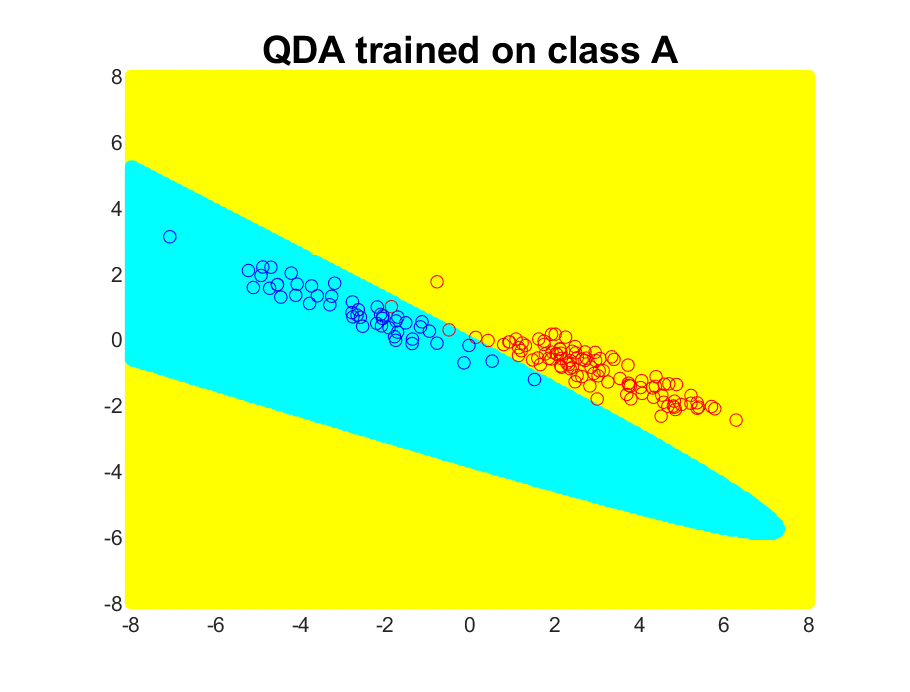
\includegraphics[scale=0.6]{qda_a.eps}
		\caption{QDA training on class A}
		\label{fig:qda_a}
	\end{figure}
	\begin{figure}
		\centering
		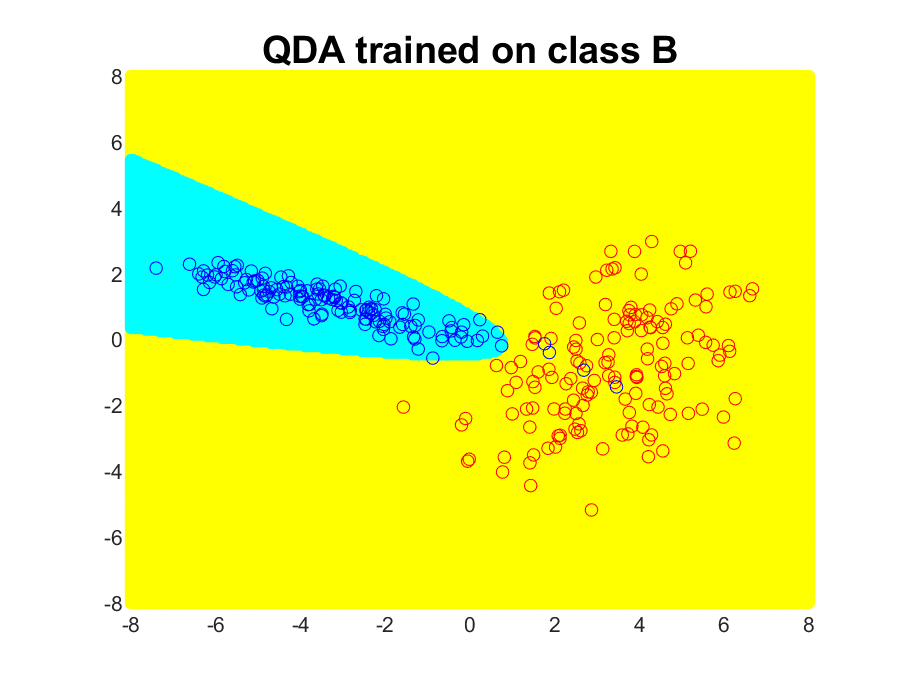
\includegraphics[scale=0.6]{qda_b.eps}
		\caption{QDA training on class B}
		\label{fig:qda_b}
	\end{figure}
	\begin{figure}
		\centering
		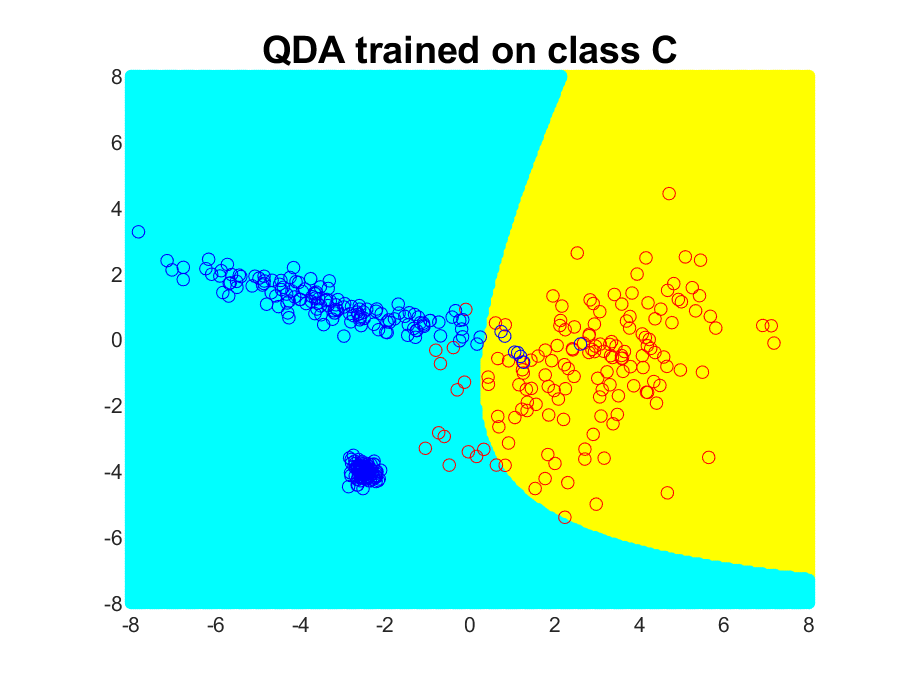
\includegraphics[scale=0.6]{qda_c.eps}
		\caption{QDA training on class C}
		\label{fig:qda_c}
	\end{figure}
	\subsection{Question (c)}
	Error:
	\begin{center}
		\begin{tabular}{ c | c | c | c | c | c | c }
			\hline
			& A train & A test & B train & B test & C train & C test \\ \hline
			LDA & 2/150 & 30/1500 & 9/300 & 83/2000 & 22/400 & 127/3000 \\ \hline
			Logistic & 0/150 & 53/1500 & 6/300 & 86/2000 & 16/400 & 68/3000  \\ \hline
			Linear & 2/150 & 31/1500 & 9/300 & 83/2000 & 22/400 & 127/3000  \\ \hline
			QDA & 1/150 & 28/1500 & 7/300 & 47/2000 & 21/400 & 121/3000 \\ \hline
		\end{tabular}
	\end{center}

	\subsection{Question (d)}
	QDA has much better performance on class B because in class B we have two gaussian with different covariances.
\end{document}
